\documentclass[a4paper,10pt]{report}\input{../0.Préambule/Préambule_cours_prof}\begin{document}

\definecolor{titlecolor}{rgb}{0.81, 0.09, 0.13}
\newpage
\setcounter{chapter}{9}
\chapter{Statistiques}

\section{Moyenne d'une série statistique}

\begin{dft}
Pour calculer la moyenne $M$ d'une série statistique, on additionne toutes les valeurs du caractère de la série puis on divise la somme obtenue par le nombre de valeurs de la série.

\noindent Si $x_1$, $x_2$, $\dots$, $x_p$ représentent les valeurs du caractère de la série, on a alors : $$M=\dfrac{x_1 + x_2 + \dots + x_p}{p}$$

\end{dft}

\begin{ex}
On cherche à déterminer la moyenne de nouveau cas de SARS-COV-2 pour la semaine du $23$ janvier au $30$ janvier.
\begin{center}
\renewcommand{\arraystretch}{1.5}
\begin{tabularx}{\linewidth}{|p{3cm}|*{7}{>{\centering \arraybackslash}X|}}
\hline
\cellcolor{lightgray!50}{Jour} & $23/01$ & $24/01$ & $25/01$ & $26/01$ & $27/01$ & $28/01$ & $29/01$ \\\hline
\cellcolor{lightgray!50}{Nombre de cas} & $\np{23 924}$ &	$\np{18 436}$ &	$\np{4 240}$ &	$\np{22 086}$ & $\np{26 916}$ & $\np{23 770}$ & $\np{22 858}$ \\\hline
\end{tabularx}
\end{center}
\noindent\grandscarreaux{\linewidth}{2.4cm}
\end{ex}

\section{Moyenne pondérée d'une série statistique}

\begin{dft}
Pour calculer la moyenne pondérée $M$ d'une série statistique, on effectue le produit de chacun des effectifs par la valeur du caractère associée, on additionne les produits et on divise la somme obtenue par l'effectif total de la série.

\noindent Si $n_1$, $\dots$, $n_p$ sont les effectifs des valeurs du caractère $x_1$, $x_2$, $\dots$, $x_p$ les valeurs associées et $N$ l'effectif total, alors : $$M=\dfrac{n_1 \times x_1 + n_2 \times x_2 + \dots + n_p \times x_p}{N}$$
\end{dft}

\begin{ex}
On cherche à déterminer le nombre de frères et sœurs qu'il y a en moyenne dans cette classe de $4^{eme}$.

\begin{center}
\renewcommand{\arraystretch}{1.5}
\begin{tabularx}{\linewidth}{|p{4cm}|*{6}{>{\centering \arraybackslash}X|}}
\hline
\cellcolor{lightgray!50}{Nombres Frères /sœurs} & $0$ & $1$ & $2$ & $3$ & $4$ & $5$ \\\hline
\cellcolor{lightgray!50}{Effectifs} & & & & & & \\\hline
\end{tabularx}
\end{center}
\noindent Calcule le nombre de frères et sœurs moyen dans votre classe de $4^{eme}$.

\noindent\grandscarreaux{\linewidth}{2.4cm}
\end{ex}

\section{Représentation d'une série statistique}

\subsection{Représentation d'une évolution}

\begin{ex}

\vspace{-8mm}
\begin{minipage}{9cm}
\vspace{5mm}
Le tableau ci-dessous donne les émissions de gaz à effet de serre en France.

\medskip
\renewcommand{\arraystretch}{1.5}
\begin{tabularx}{9cm}{|p{4.5cm}|*{4}{>{\centering \arraybackslash}X|}}
\hline
\cellcolor{lightgray!50}{Année} & $2000$ & $2010$ & $2015$ & $2017$ \\\hline
\cellcolor{lightgray!50}{Millions de tonnes de $CO_2$} & $543$ & $499$ & $447$ & $452$ \\\hline
\end{tabularx}

\medskip
\noindent Le diagramme en bâtons ci-contre représente l'évolution des émissions de $CO_2$ par an.

\medskip
\noindent Rappel : La hauteur de chaque bâton est proportionnelle à l'effectif de la valeur qu'il représente.
\end{minipage}
\begin{minipage}{9cm}
\begin{center}
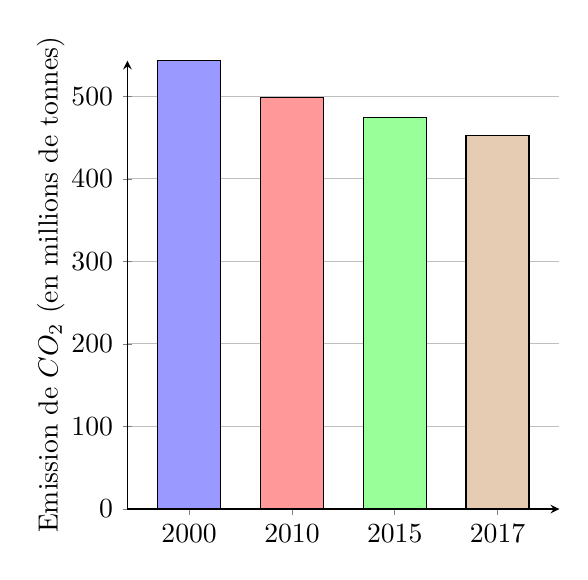
\begin{tikzpicture}
\begin{axis}[symbolic x coords={2000, 2010, 2015, 2017},
ymin=0,
xscale=0.8,
xtick=data,
ylabel=Emission de $CO_2$ (en millions de tonnes),
ymajorgrids,
axis x line=bottom,axis y line = left,
enlarge x limits=0.2,
]
\addplot[ybar,fill=blue!40,bar width=1cm] coordinates { (2000,  543) (2010,  499) (2015,  474) (2017,  452) };
\addplot[ybar,fill=red!40,bar width=1cm] coordinates {(2010,  499) };
\addplot[ybar,fill=green!40,bar width=1cm] coordinates {(2015,  474)};
\addplot[ybar,fill=brown!40,bar width=1cm] coordinates {(2017,  452) };
\end{axis}
\end{tikzpicture}
\end{center}
\end{minipage}
\end{ex}

\vspace{-5mm}
\subsection{Représentation d'une répartition}

\begin{ex}
\begin{minipage}{7cm}
\begin{center}
\begin{tikzpicture}[scale=2]

\newcounter{a}
\newcounter{b}
\foreach \p/\t/\r in {78/Azote/blue!40, 21/Oxygène/red!40, 1/Autres/brown!40}
  {
    \setcounter{a}{\value{b}}
    \addtocounter{b}{\p}
    \slice{\thea/100*360}
          {\theb/100*360}
          {\large{\textbf{\p $\%$}}}{\large{\textbf{\textcolor{\r}{\t}}}}{\r}
  }
\end{tikzpicture}
\end{center}
\end{minipage}
\begin{minipage}{10cm}
Le tableau ci-dessous donne la composition en gaz de l'atmosphère terrestre.
\medskip
\begin{center}
\renewcommand{\arraystretch}{1.5}
\begin{tabularx}{\linewidth}{|p{3cm}|*{3}{>{\centering \arraybackslash}X|}}
\hline
\cellcolor{lightgray!50}{Gaz} & Azote & Oxygène & Autres Gaz \\\hline
\cellcolor{lightgray!50}{Composition}	& $78\%$ & $21\%$ & $1\%$ \\\hline
\end{tabularx}
\end{center}

\medskip
\noindent Le diagramme circulaire ci-contre représente la répartition des gaz de l'atmosphère terrestre.

\medskip
\noindent Rappel : La mesure de l'angle de chaque secteur est proportionnelle à l'effectif (et à la fréquence) de la valeur qu'il représente.
\end{minipage}
\end{ex}

\begin{rmq}
Pour calculer ces mesures d'angles, on utilise un tableau de proportionnalité.
\begin{center}
\renewcommand{\arraystretch}{2.2}
\begin{tabularx}{\linewidth}{|p{3cm}|*{4}{>{\centering \arraybackslash}X|}}
\hline
\cellcolor{lightgray!50}{Gaz} & Azote & Oxygène & Autres Gaz & Total\\\hline
\cellcolor{lightgray!50}{Composition}	& $78\%$ & $21\%$ & $1\%$ & $100\%$\\\hline
\cellcolor{lightgray!50}{Mesure de l'angle} &  &  &  &  \\\hline
\end{tabularx}
\end{center}

\noindent\grandscarreaux{\linewidth}{4cm}
\end{rmq}

\newpage
\section{Médiane et étendue}
	
\begin{dft}
L'étendue d'une série statistique est la différence entre la plus grande et la plus petite des valeurs prises par cette série.
\end{dft}	
	
\begin{dft}
On appelle médiane $Me$ d'une série statistique dont les valeurs sont ordonnées, tout nombre qui partage cette série en deux sous séries de même effectif.
\end{dft}

\begin{ex}
Voici le temps consacré, en minutes, au petit-déjeuner par $16$ personnes.
\begin{center}
\renewcommand{\arraystretch}{2}
\begin{tabularx}{\linewidth}{|*{16}{>{\centering \arraybackslash}X|}}
\hline
$16$ & $12$ & $1$ & $9$ & $17$ & $19$ & $13$ & $10$ & $4$ & $8$ & $7$ & $8$ & $14$ & $12$ & $14$ & $9$\\\hline
\end{tabularx}
\end{center}

\noindent Détermine une valeur médiane ainsi que l'étendue de cette série statistique.

Étape 1 : Ranger les valeurs dans l'ordre croissant :

\noindent\grandscarreaux{\linewidth}{4cm}
Étape 2 : Déterminer l'étendue de la série

\noindent\grandscarreaux{\linewidth}{4cm}
Étape 3 : Déterminer la médiane de la série

\noindent\grandscarreaux{\linewidth}{4cm}
\end{ex}

\end{document}